\chapter{Obtaining and Solving the Hubbard Model Approximately and in Simple Limits}
\label{ap:hubbardObSol}

\pagebreak

\section{Hartree-Fock Approximation and the Self Consistent Field Method}\label{sec:hartree-fock}

In the mean field approximation, the quartic term of the interaction part of the Hamiltonian

\begin{equation*}
V_{\text{int}} = \frac{1}{2} V^{\nu\mu}_{\nu'\mu'} c_\nu^\dagger c_\mu^\dagger c_{\mu'} c_{\nu'} ,
\end{equation*} 
becomes a sum of all possible 2-body terms (note that terms of the type $\left\langle cc \right\rangle$ and $\left\langle c^\dagger c^\dagger \right\rangle$ must vanish since they do not conserve the number of particles).

\begin{equation}\label{eq:c_mft}
c_\nu^\dagger c_\mu^\dagger c_{\mu'} c_{\nu'} \approx - \left\langle c_\nu^\dagger c_{\mu'} \right\rangle  c_{\mu}^\dagger c_{\nu'} - \left\langle c_{\mu}^\dagger c_{\nu'} \right\rangle c_{\nu}^\dagger c_{\mu'} + \left\langle c_{\nu}^\dagger c_{\nu'} \right\rangle  c_{\mu}^\dagger c_{\mu'} + \left\langle c_{\mu}^\dagger c_{\mu'} \right\rangle  c_{\nu}^\dagger c_{\nu'} ,
\end{equation}
where we ignored the constant terms which are unimportant in the Hamiltonian, in what concerns the dynamics. 

This Hartree-Fock, or mean field approximation is slightly tricky to obtain. It requires one to be precise about what the meaning of the mean field approximation is in terms of creation and annihilation operators. In mean field theory, we assume that the operator

\begin{equation}
\rho_{\mu\mu'} = c_{\mu}^\dagger c_{\mu'}
\end{equation}
is close to its average, so that we neglect second order terms in the fluctuations $\delta \rho_{\mu\mu'}$, i.e. $\rho_{\mu\mu'}$ is \say{large} only when its average is nonzero, otherwise it is negligibly small. Thus, for most combinations of indices, this operator will vanish. We follow the usual mean field procedure of writing the original operator as a deviation plus an average

\begin{equation}\label{eq:hartree}
c_{\nu}^\dagger \bigg( c_\mu^\dagger c_{\mu'} - \left\langle c_\mu^\dagger c_{\mu'} \right\rangle \bigg) c_{\nu'} + c_{\nu}^\dagger c_{\nu'} \left\langle c_\nu^\dagger c_{\nu'} \right\rangle
\end{equation}

Then we note that if $\nu' \neq \mu$, we can commute $c_{\nu'}$ with the parenthesis. But this is true except in a set of measure zero. In the thermodynamic limit $N \rightarrow \infty$, the number of allowed $\bm k$-states is very large, and if we take a continuum limit in which the set of possible $\bm k$-states becomes dense, then the commutation becomes exact. Repeating the procedure of writing (\ref{eq:hartree}) replacing $c_\nu^\dagger c_{\nu'} \mapsto c_\nu^\dagger c_{\nu'} - \left\langle c_\nu^\dagger c_{\nu'} \right\rangle + \left\langle c_\nu^\dagger c_{\nu'} \right\rangle $, we obtain

\begin{equation}\label{eq:mf}
\underbrace{\big( c_\nu^\dagger c_{\nu'} - \left\langle c_\nu^\dagger c_{\nu'} \right\rangle \big) \big( c_\mu^\dagger c_{\mu'} - \left\langle c_\mu^\dagger c_{\mu'} \right\rangle \big)}_{\propto \, \delta \rho_{\mu\mu'} \, \delta \rho_{\nu\nu'} \rightarrow 0} + c_\nu^\dagger c_{\nu'} \left\langle c_\mu^\dagger c_{\mu'} \right\rangle + c_\mu^\dagger c_{\mu'} \left\langle c_\nu^\dagger c_{\nu'} \right\rangle - \left\langle c_\mu^\dagger c_{\mu'} \right\rangle \left\langle c_\nu^\dagger c_{\nu'} \right\rangle
\end{equation}

But this result is not complete. This is only the so called Hartree or direct term. Due to identical nature of the interacting electrons, we must consider an analogous contribution for $\left\langle c_\nu^\dagger c_{\mu'} \right\rangle$ finite. We start by exchanging the first two operators: 

\begin{equation}
c_\nu^\dagger c_\mu^\dagger c_{\mu'} c_{\nu'} = - c_\mu^\dagger c_\nu^\dagger c_{\mu'} c_{\nu'}
\end{equation}
Then we proceed in exactly the same manner as before. The result is analogous, but a minus sign appears and we must switch $\mu \leftrightarrow \nu$:

\begin{equation}
- c_\mu^\dagger c_{\nu'} \left\langle c_\nu^\dagger c_{\mu'} \right\rangle \\
- c_\nu^\dagger c_{\mu'} \left\langle c_\mu^\dagger c_{\nu'} \right\rangle + \left\langle c_\nu^\dagger c_{\mu'} \right\rangle \left\langle c_\mu^\dagger c_{\nu'} \right\rangle
\end{equation}

Ignoring the constant terms of the type $\left\langle c^\dagger c \right\rangle \left\langle c^\dagger c \right\rangle$, we recover equation (\ref{eq:c_mft}).

Now we can simply substitute the mean field expansion of equation (\ref{eq:c_mft}) in the second term to  obtain the last term that is subtracted in equation (\ref{eq:startingHamiltonian}) (we omit the boldface on the $\bm k$'s solely in the following equation, but keep in mind that they are vectors):

\begin{equation}\label{eq:mean_field}
\begin{split}
&\frac{1}{2} \sum_{\substack{ k_1 k_2 k_1' k_2' \\ \sigma_1 \sigma_2} } V^{k_1 k_2}_{k_1' k_2'} \bigg( - \underbrace{\left\langle c_{k_1 \sigma_1}^\dagger c_{k_2' \sigma_2} \right\rangle}_{\delta_{k_1 k_2'} \delta_{\sigma_1 \sigma_2} f_{k_1} } c_{k_2 \sigma_2}^\dagger c_{k_1' \sigma_1}  - \underbrace{\left\langle c_{k_2 \sigma_2}^\dagger c_{k_1' \sigma_1}  \right\rangle}_{\delta_{k_2 k_1'} \delta_{\sigma_1 \sigma_2} f_{k_2} } c_{k_1 \sigma_1}^\dagger c_{k_2' \sigma_2} + \underbrace{\left\langle c_{k_1 \sigma_1}^\dagger c_{k_1' \sigma_1} \right\rangle}_{\delta_{k_1 k_1'} f_{k_1} } c_{k_2 \sigma_2}^\dagger c_{k_2' \sigma_2}  \\
& + \underbrace{\left\langle c_{k_2 \sigma_2}^\dagger c_{k_2' \sigma_2} \right\rangle}_{\delta_{k_2 k_2'} f_{k_2} } c_{k_1 \sigma_1}^\dagger c_{k_1' \sigma_1} \bigg)\\
\end{split}
\end{equation}

In the language of Hartree Fock theory, the first two terms give the exchange term, and the last two terms the direct term. Apart from the $\frac{1}{2}$ factor, the term in (\ref{eq:mean_field}) becomes

\begin{equation}
\begin{split}
&- \sum_{\substack{k_1 k_2 \\ k_1' \sigma_1}} V_{k_1' k_1}^{k_1 k_2} f_{k_1} c_{k_2 \sigma_1}^\dagger c_{k_1' \sigma_1}  - \sum_{\substack{k_1 k_2 \\ k_2' \sigma_1}} V_{k_2 k_2'}^{k_1 k_2} f_{k_2} c_{k_1 \sigma_1}^\dagger c_{k_2' \sigma_1} + \sum_{\substack{k_1 k_2 k_2' \\ \sigma_1 \sigma_2}} V_{k_1 k_2'}^{k_1 k_2} f_{k_1} c_{k_2 \sigma_2}^\dagger c_{k_2' \sigma_2} \\
& + \sum_{\substack{k_1 k_2 k_1' \\  \sigma_1 \sigma_2}} V_{k_1' k_2'}^{k_1 k_2} f_{k_2} c_{k_1 \sigma_1}^\dagger c_{k_1' \sigma_1} \\
&= \sum_{k_1 k_2 \sigma_1} \bigg( 4 V_{k_1 k_2}^{k_1 k_2} - 2  V_{k_2 k_1}^{k_1 k_2}  \bigg) f_{k_2} c_{k_1 \sigma_1}^\dagger c_{k_1 \sigma_1}
,
\end{split}
\end{equation}
where we used momentum conservation to eliminate a $k'$-sum. Moreover, we used that the sum on spin ($\pm 1/2$) on the last two terms gives factors of 2 , since the interaction is spin independent and thus no spin-dependent term remains after we use momentum conservation. Making $k_1 \rightarrow k , \, k_2 \rightarrow k', \, \sigma_1 \rightarrow \sigma$, and recalling the definition in equation (\ref{eq:integrals}), we obtain the result we sought.

The procedure above is meant to serve as an intuitive derivation. Now we approach the problem more formally. In fact, the argument that allowed us to perform the commutation leading to equation \ref{eq:mf} seems somewhat handwaving. We should not have to take the thermodynamic limit to perform a mean field expansion. A more systematic procedure to obtain the mean field expansion of a quartic interaction term was given by Pierre de Gennes in the context of a mean field treatment of a superconductor in a magnetic field \cite{gennes_superconductivity_1999}. Our case is actually much simpler to analyze, but we follow the same argument as de Gennes.

Consider the Hamiltonian to be given by $\mathcal{H} = \mathcal{H}_0 + \mathcal{H}_1$, where

\begin{equation}
\begin{split}
\mathcal{H}_0 &= \sum_{\bm k, \sigma} \varepsilon_{\bm k} c_{\bm k, \sigma}^\dagger c_{\bm k, \sigma} \\
\mathcal{H}_1 &= \frac{1}{2} \sum_{\substack{\bm k_1 \bm k_2 \\ \bm k_1' \bm k_2' \\  \sigma_1 \sigma_2}} V_{k_1' k_2'}^{k_1 k_2} c_{\bm k_1 \sigma_1}^\dagger c_{\bm k_2 \sigma_2}^\dagger c_{\bm k_2' \sigma_2} c_{\bm k_1' \sigma_1} 
\end{split}
\end{equation}

We would like to find an effective Hamiltonian that is quadratic in the fermion operators:

\begin{equation}
\mathcal{H}_{\text{eff}} = \sum_{\bm k, \sigma} (\varepsilon_{\bm k} + v_{\bm k} ) c_{\bm k, \sigma}^\dagger c_{\bm k, \sigma}
\end{equation}

This effective Hamiltonian is diagonal, so assuming we know $v_{\bm k}$ (which is what we are trying to determine in the first place), we can compute its eigenstates $\{ \left| \phi \right\rangle \}$, and compute the average of the actual Hamiltonian $\mathcal{H}$ using the basis $\{ \left| \phi \right\rangle \}$:

\begin{equation}\label{eq:avH}
\left\langle \mathcal{H} \right\rangle = \frac{\sum_\phi \left\langle \phi | \mathcal{H} | \phi \right\rangle e^{-\beta E_\phi} }{\sum_\phi e^{-\beta E_\phi} }
\end{equation}

Our criterion to determine $\mathcal{H}_{\text{eff}}$ is the requirement that the free energy $F = \left\langle \mathcal{H} \right\rangle - TS$, with the average computed with the eigenstates of $\mathcal{H}_{\text{eff}}$ be stationary, i.e. $\delta F = 0$. Thus, we find the mean field form of the quartic term invoking only a variational principle without any need to resort to the thermodynamic limit. In fact, we never even have to explicitly compute the average in equation (\ref{eq:avH}). In terms of pairs of fermion operator averages, we have 

\begin{equation}
\left\langle \mathcal{H} \right\rangle = \sum_{\bm k, \sigma} \varepsilon_{\bm k} \left\langle c_{\bm k, \sigma}^\dagger c_{\bm k, \sigma} \right\rangle + \frac{1}{2} \sum_{\substack{\bm k_1 \bm k_2 \\ \bm k_1' \bm k_2' \\  \sigma_1 \sigma_2}} V_{k_1' k_2'}^{k_1 k_2} \left\langle c_{\bm k_1 \sigma_1}^\dagger c_{\bm k_2 \sigma_2}^\dagger c_{\bm k_2' \sigma_2} c_{\bm k_1' \sigma_1} \right\rangle ,
\end{equation}
where the last term can be reduced to products of averages of pairs of fermion operators by Wick's theorem:

\begin{equation}
\begin{split}
&\left\langle c_{\bm k_1 \sigma_1}^\dagger c_{\bm k_2 \sigma_2}^\dagger c_{\bm k_2' \sigma_2} c_{\bm k_1' \sigma_1} \right\rangle = \left\langle c_{\bm k_1 \sigma_1}^\dagger c_{\bm k_1' \sigma_1} \right\rangle  \left\langle c_{\bm k_2 \sigma_2}^\dagger c_{\bm k_2' \sigma_2} \right\rangle - \left\langle c_{\bm k_1 \sigma_1}^\dagger c_{\bm k_2' \sigma_2} \right\rangle  \left\langle c_{\bm k_2 \sigma_2}^\dagger c_{\bm k_1' \sigma_1} \right\rangle \\
& + \left\langle c_{\bm k_1 \sigma_1}^\dagger c_{\bm k_2 \sigma_2}^\dagger \right\rangle \left\langle c_{\bm k_2' \sigma_2} c_{\bm k_1' \sigma_1} \right\rangle
\end{split}
\end{equation}

The computation is now done by using the rules (for all $\bm k$ and $\sigma$).

\begin{equation}\label{eq:rules}
\begin{split}
\left\langle c_{\bm k, \sigma}^\dagger c_{\bm k', \sigma'} \right\rangle &= \delta_{\bm k, \bm k'} \delta_{\sigma, \sigma'} f_{\bm k} \\
\left\langle c_{\bm k, \sigma}^{(\dagger)} c_{\bm k', \sigma'}^{(\dagger)} \right\rangle &= 0 ,
\end{split}
\end{equation}
where $f_{\bm k} = (e^{\beta(\varepsilon_{\bm k} - \mu)} +1 )^{-1}$ is the Fermi-Dirac function.

Since the original Hamiltonian is quadratic, again we have that terms of the type $\left\langle cc \right\rangle$ and $\left\langle c^\dagger c^\dagger \right\rangle$ do not contribute. Hence, varying the free energy, we obtain

\begin{equation}
\begin{split}
&\delta F =  \delta \left\langle \mathcal{H} \right\rangle - T \delta S = \sum_{\bm k \sigma} \varepsilon_{\bm k} \delta \left\langle c_{\bm k, \sigma}^\dagger c_{\bm k, \sigma} \right\rangle + \frac{1}{2} \sum_{\substack{\bm k_1 \bm k_2 \\ \bm k_1' \bm k_2' \\  \sigma_1 \sigma_2}} V_{k_1' k_2'}^{k_1 k_2} \bigg( \left\langle c_{\bm k_1 \sigma_1}^\dagger c_{\bm k_1' \sigma_1} \right\rangle \delta  \left\langle c_{\bm k_2 \sigma_2}^\dagger c_{\bm k_2' \sigma_2} \right\rangle + \\
&\delta \left\langle c_{\bm k_1 \sigma_1}^\dagger c_{\bm k_1' \sigma_1} \right\rangle  \left\langle c_{\bm k_2 \sigma_2}^\dagger c_{\bm k_2' \sigma_2} \right\rangle  - \left\langle c_{\bm k_1 \sigma_1}^\dagger c_{\bm k_2' \sigma_2} \right\rangle  \delta \left\langle c_{\bm k_2 \sigma_2}^\dagger c_{\bm k_1' \sigma_1} \right\rangle - \delta \left\langle c_{\bm k_1 \sigma_1}^\dagger c_{\bm k_2' \sigma_2} \right\rangle  \left\langle c_{\bm k_2 \sigma_2}^\dagger c_{\bm k_1' \sigma_1} \right\rangle \bigg) - T \delta S ,
\end{split}
\end{equation}
which can be simplified exactly in the same manner as in equation (\ref{eq:mean_field}), i.e. by using the rules of equation (\ref{eq:rules}), and that the occupation of a given momentum state $\bm k$ is given by the Fermi-Dirac function:

\begin{equation}
\delta F = \sum_{\bm k \sigma} \varepsilon_{\bm k} \delta \left\langle c_{\bm k, \sigma}^\dagger c_{\bm k, \sigma} \right\rangle + \sum_{\bm k \bm k' \sigma} \bigg( 2 V_{\bm k \bm k'}^{\bm k \bm k'} -  V_{\bm k' \bm k}^{\bm k \bm k'}  \bigg) f_{\bm k'} c_{\bm k \sigma} \delta \left\langle c_{\bm k, \sigma}^\dagger c_{\bm k, \sigma} \right\rangle
\end{equation}

We can now compare $\delta F = \delta \left\langle \mathcal{H} \right\rangle - T \delta S$ and $\delta F' = \delta \left\langle \mathcal{H}_{\text{eff}} \right\rangle - T \delta S$, which is simply given by

\begin{equation}
\delta F' =  \delta \left\langle \mathcal{H}_{\text{eff}} \right\rangle - T \delta S = \sum_{\bm k \sigma} (\varepsilon_{\bm k} + v_{\bm k}) \delta \left\langle c_{\bm k, \sigma}^\dagger c_{\bm k, \sigma} \right\rangle
\end{equation}

Requiring both free energies to be stationary, we find our desired result

\begin{equation}
v_{\bm k} = \sum_{\bm k'} \bigg( 2 V_{\bm k \bm k'}^{\bm k \bm k'} -  V_{\bm k' \bm k}^{\bm k \bm k'}  \bigg) f_{\bm k'} ,
\end{equation}
which agrees with the result obtained from our initial more intuitive, but somewhat less rigorous  argument.

\section{Mott insulators}\label{sec:mott}

Band theory was found to be flawed soon after it was introduced.
The picture it proposes is simple and generally works pretty well.
It is based on considering the electrons to be independently moving under the constant background potential created by the ions.
The solutions of the Schr\"odinger for free electrons in a periodic potential $U(\bm r)$, such that $U(\bm r) = U(\bm r + \bm R)$,

\begin{equation}\label{eq:schrodinger}
\bigg[ -\frac{1}{2m} \nabla^2 + U(\bm r) \bigg] \psi (\bm r) = \varepsilon \psi (\bm r)
\end{equation}
are given by Bloch's theorem: $\psi_{\bm k} (\bm r) = e^{i\bm k \cdot \bm r} u_{\bm k} (\bm r)$.
Note that we made $\hbar = 1$.
Replacing this wave function in equation (\ref{eq:schrodinger}), we obtain a differential equation for $u_{\bm k} (\bm r)$, which has in general an infinite number of solutions.
We label them with an index $n$, which we call the band index.
To each solution there corresponds a function $\varepsilon_{n\bm k}$.
The set of these functions is known as the band structure.
Since electrons are taken to be independent in band theory, the N-electron eigenstates are obtained by placing an electron in each quantum state.
Each state is labelled by its energy $\varepsilon_{n\bm k \sigma}$.
Since our model Hamiltonian does not couple spins (via an electron interaction, for example) and assuming there is no external magnetic field and that the system has an inversion center, we have $\varepsilon_{n\bm k \uparrow} = \varepsilon_{n\bm k \downarrow}$.
In general there might be energies for which there is no corresponding $\varepsilon_{n\bm k \sigma}$.
These form intervals called forbidden bands\footnote{We disregard surface states that may have energies that fall in the forbidden bands of band theory.}.
Thus, the ground state of our model may be obtained by filling the energy levels starting from the lowest energy state.
Two cases are particularly relevant:
\begin{itemize}
\item Every band is either fully occupied or empty.
The first excited state differs from the ground state by $\Delta$, the separation between the last fully occupied band and the first empty band.
It is then impossible to induce the motion of the electrons by applying an arbitrarily small voltage.
This is what it means to be an \emph{insulator}.
Since there $2N$ states per band, this is not possible unless the number of electrons per unit cell is an even integer.
\item One or more of the bands are partially filled.
The energy of occupied state of higher energy is named the Fermi energy $\varepsilon_F$.
In this case, the separation between the ground state and the first excited state tends to $0$ in the thermodynamic limit, $N \rightarrow \infty$.
The system may then respond to infinitesimal excitations, which is the definition of a metal.
\end{itemize}

Band theory made it possible to predict whether a solid would be a metal or an insulator.
However, its success rests crucially on the independent electron approximation.
Thus, it is not surprising that for compounds with strongly correlated electrons the theory might fail \cite{mila_physique_2007}.
The Coulomb interaction is in general non negligible, and the effects it leads to are not captured by a mean field approach.
One must resort to many-body theory.
An example of a many-body effect that band theory doesn't capture is  superconductivity.
However, this does not deem band theory useless.
In fact, the superconducting phase arises due to an instability of a state that is itself well described by band theory \cite{gennes_superconductivity_1999}.
A far greater failure of band theory is that predicts certain compounds with an odd number of electrons per unit cell, such as \chem{NiO} and \chem{La_2 Cu O_4},  to be metals, while in fact  they turn out to be (Mott) insulators.
Mott devised a simple argument to justify this failure.
It is based on considering the elementary electronic excitations of a solid composed by hydrogen atoms as a function of the distance between atoms.

Consider a hypothetical solid consisting of a square lattice with hydrogen atoms on its points.
Each unit cell has one hydrogen atom, and consequently one electron.
Band theory would predict such a solid to be a metal.
However, if the lattice parameter $a$ is large enough, the solid cannot remain a metal.
There must be some value of the lattice parameter $a = a_c$ for which the system becomes an insulator.
When current flows through a sample of this solid, electrons hop consecutively, reaching positions that can be quite far on the lattice.
For a metal, this process occurs even when exciting the system with an infinitesimal amount of energy.
How much energy do we need to provide for this process to occur?

\begin{figure}[ht!]\label{hubbardOneHoleOneDoublyOc}
\centering
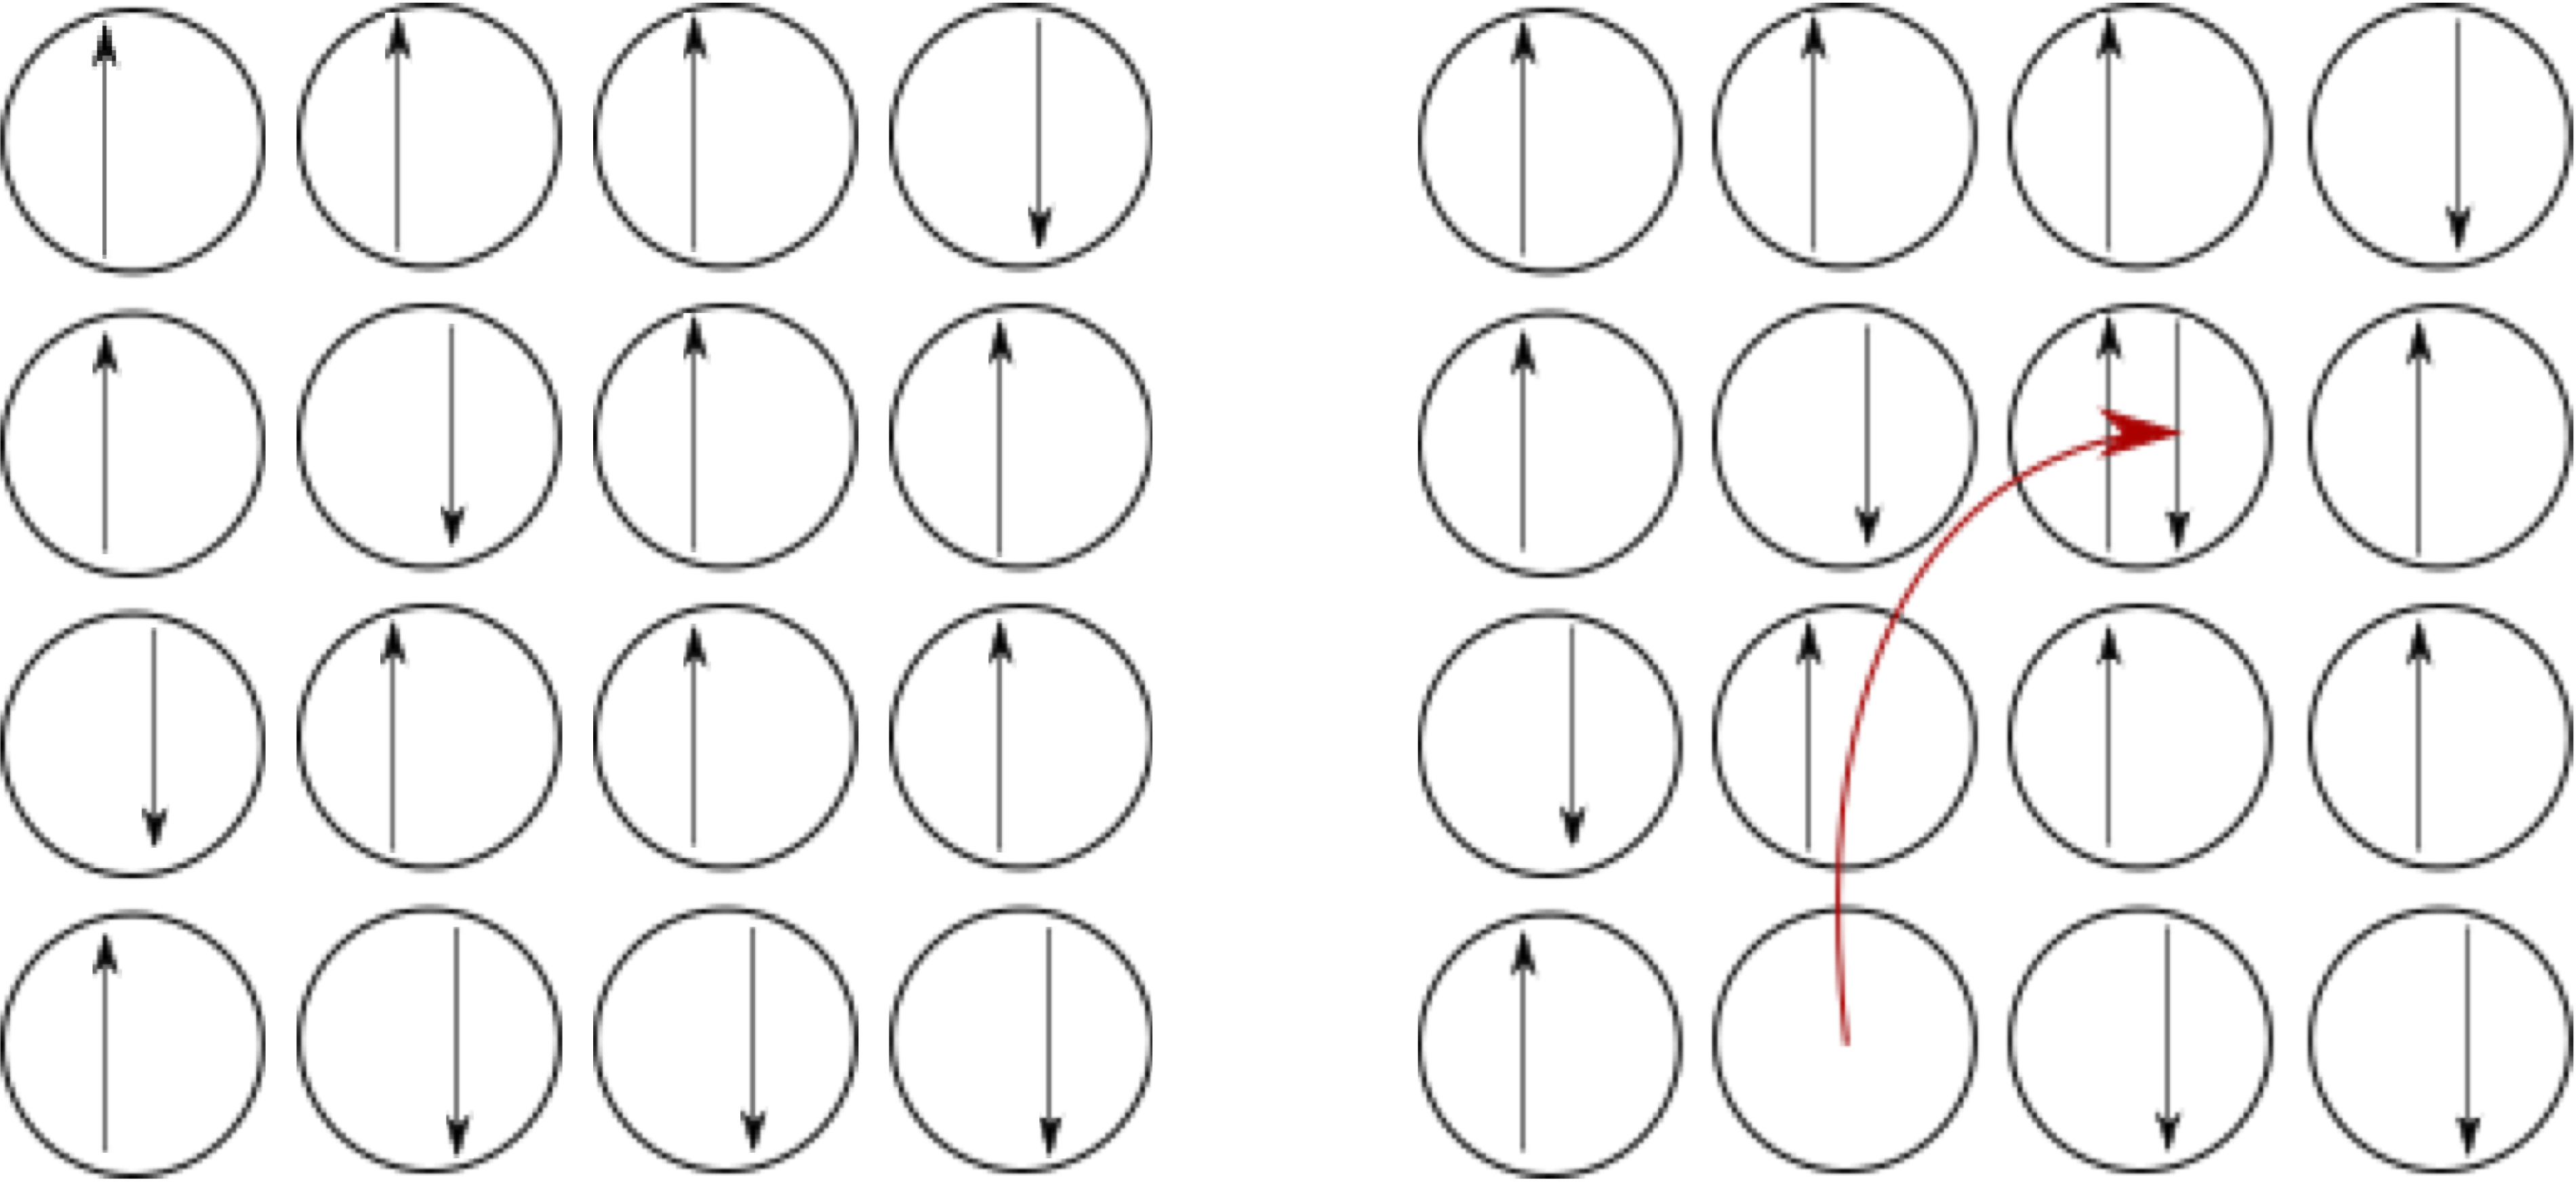
\includegraphics[width = 9cm]{Hubbard/hubbardOneHoleOneDoublyOcV2.png}
\caption[Configuration of the Hubbard model on the square lattice with a hole and a doubly occupied site.]{On the right, a configuration of hydrogen atoms on a square lattice with a hole and a doubly occupied site obtained by delocalization of the spin down electron on the left.}
\end{figure}

If $a$ is large, we have essentially one electron per site at the start.
When an electron is displaced, we end up with a hole and a doubly occupied site.
The potential energy of such a state is

\begin{equation}
E_{H^-} + E_{H^+} - 2 E_H 
\end{equation}

Due to the Coulomb repulsion between the two electrons in $H^-$, this quantity is strictly positive.
Call it $U > 0$.
On the other hand, the system also has kinetic energy: both the hole and the doubly occupied site can delocalize.
Let $W$ be the bandwidth corresponding to the delocalization of an electron on the lattice.
Both the hole and the doubly occupied will stay at the bottom of the band and gain an energy $W/2$ (assuming that this delocalization is of the same order of magnitude).
The dominant transfer integral $-t$ is between nearest neighbors.
The dispersion relation then reads

\begin{equation}
\varepsilon_{\bm k} = -2 t ( \cos k_x + \cos k_y ) 
\end{equation}

The bandwidth is then $W = 8 t$.
The energy of a configuration with a hole and a doubly occupied site is

\begin{equation}
\Delta_c = U - W ,
\end{equation}
where $U$ is practically independent of the lattice parameter $a$.
The bandwidth $W$, however, depends strongly on $a$.
When $a \gg a_0$, where $a_0$ is the Bohr radius, the transfer integral is exponentially small, because only the exponential tails of the wave functions are relevant.
In this limit, $\Delta_c \approx U$ is a large, positive number, and the system is an insulator.
This type of insulator is called a Mott insulator, and $\Delta_c$ is called the charge gap.
As $a$ decreases, $t$ increases, and there must be a critical value $a_c \sim a_0$, for which $U = W$.
Below this value, the computation of $\Delta_c$ is not valid anymore because the gap cannot be negative.
Thus, there must be a metal-insulator transition.
It is possible to see this transition if we apply enough pressure to a Mott insulator so as to decrease $a$ and increase $t$.
A transition of this type was first seen in the 1970's for $V_2 O_3$\footnote{Of course, the transition is not so easy to describe. We should consider the Hubbard model!
However, this simple argument provides an intuitive picture.}.
There is a fundamental difference between a band insulator and a Mott insulator.
While we must pay an energy $\Delta_c$ to make a charge excitation, there is no cost for making a spin excitation: we can flip the spin of an electron without creating a doubly occupied site.
The fluctuations of both charge and spin due to the electron interactions may then lead to magnetic behavior characteristic of correlated  systems.

\section{Computing the partition function for a quadratic Hamiltonian}
\label{sec:Zquadratic}

Let us start by restating the result we want to prove.

If $\mathcal{H} = \bm c^\dagger \bm H \bm c$, where $\bm H$ is a $N \times N$ Hermitian matrix, then we have that

\begin{equation}\label{eq:apZquadratic}
\text{Tr} \big[ e^{-\beta \mathcal{H} } \big] = \prod_{i=1}^N ( 1 + e^{-\beta \lambda_{i} } ) ,
\end{equation}
where $\lambda_{i}$ are the eigenvalues of $\bm H$. 

We will now prove equation (\ref{eq:apZquadratic}). Without loss of generality, let us consider $\bm H$ to be diagonal. Then, its eigenvalues coincide with the diagonal entries, so that $\bm H = \text{diag}(\lambda_{i} )$. The quadratic Hamiltonian may then be  diagonalized

\begin{equation*}
\mathcal{H} = {\bm c}^\dagger \text{diag} (\lambda_{1}, \lambda_{2}, .., \lambda_{N}) \bm c = \sum_{i=1}^N \lambda_{i} n_{i}
\end{equation*}

We continue by induction. When $N=1$, we have

\begin{equation}
\text{Tr} (e^{-\beta\mathcal{H} } ) = \left\langle 0 \left| e^{-\beta \lambda_{1} n_{1}}  \right| 0 \right\rangle + \left\langle 1 \left| e^{-\beta \lambda_{1} n_{1}}   \right| 1 \right\rangle = 1 + e^{-\beta \lambda_{1} }
\end{equation}

Assuming that for $N-1$:

\begin{equation*}
\text{Tr} \big[ e^{-\beta \sum_{i=1}^{N-1} \lambda_{i} n_{i} } \big] = \prod_{i=1}^{N-1} ( 1 + e^{-\beta \lambda_{i} } )
\end{equation*}
we can compute the trace for $i$ going up to $N$.

\begin{equation*}
\begin{split}
&\text{Tr} \big[ e^{-\beta \sum_{i=1}^{N-1} \lambda_{i} n_{i} } \big] = \sum_{i=1}^{N} \left\langle \psi_1^{\lambda_1} \psi_2^{\lambda_2} ... \psi_N^{\lambda_N} \left| e^{-\beta \sum_{i=1}^N \lambda_{i} n_{i}}  \right| \psi_1^{\lambda_1} \psi_2^{\lambda_2} ... \psi_N^{\lambda_N} \right\rangle \\
&= \sum_{i=1}^{N-1} \bigg( \left\langle \{\psi_i^{\lambda_i}\} 0 \left| e^{-\beta \sum_{i=1}^N \lambda_{i} n_{i}} e^{-\beta \lambda_{N} n_{N}} \right| \{\psi_i^{\lambda_i}\} 0 \right\rangle + \left\langle \{\psi_i^{\lambda_i}\} 1 \left| e^{-\beta \sum_{i=1}^N \lambda_{i} n_{i}} e^{-\beta \lambda_{N} n_{N}} \right| \{\psi_i^{\lambda_i}\} 1 \right\rangle \bigg) \\
&= (1 + e^{-\beta \lambda_{N} } ) \sum_{i=1}^{N-1} \left\langle \{\psi_i^{\lambda_i}\} \left| e^{-\beta \lambda_{i} n_{i}} \right| \{\psi_i^{\lambda_i}\} \right\rangle \\
&= (1 + e^{-\beta \lambda_{N} } ) \prod_{i=1}^{N-1} (1 + e^{-\beta \lambda_{i} } ) \\
&= \prod_{i=1}^{N} (1 + e^{-\beta \lambda_{i} } )
\end{split}
\end{equation*}

To complete the proof we note that for any $\bm H$, there exists a unitary matrix $\bm Q$, such that $\bm Q^T \bm H \bm Q = \bm \Lambda = \text{diag}(\lambda_{i})$. Let $\tilde{\bm c} = \bm Q \bm c$, and $\tilde{n_i} = \tilde{c_i}^\dagger \tilde{c_i}$. Then, we find

\begin{equation*}
\mathcal{H} = \bm c^\dagger \bm H \bm c = \bm \tilde{\bm c}^\dagger \bm \Lambda \tilde{\bm c} = \sum_{i=1}^N \lambda_{i} \tilde{n}_{i}
\end{equation*}

The trace is independent of the choice of basis functions. Thus, we have

\begin{equation*}
\begin{split}
\text{Tr} ( e^{-\beta \mathcal{H} } ) &= \text{Tr} \bigg( \prod_{i=1}^N e^{-\beta \lambda_{i} \tilde{n}_{i} } \bigg) \\
&= \prod_{i=1}^N \bigg( 1 + e^{-\beta \lambda_{i} } \bigg) \quad\quad \qedsymbol
\end{split}
\end{equation*}

\section{Density of states for a 1D tight binding model}
\label{sec:dos1d}

Using the definition of the density of states

\begin{equation}
N ( E ) = \frac{1}{N} \sum_{\bm k} \delta_{E,\varepsilon_{\bm k}} \rightarrow \frac{1}{(2\pi)^d} \int d\bm k \, \delta ( E - \varepsilon_{\bm k})\,\, \text{when}\,\, N\rightarrow \infty.
\end{equation}
with $\varepsilon_k = - 2 t \cos k$, in the thermodynamic limit we obtain

\begin{equation}
N ( E ) = \frac{1}{2\pi} \int d k \, \delta ( E + 2t \cos k)
\end{equation}

Now we use a well known property of the delta function

\begin{equation}
\delta ( g(x) ) = \sum_{ \{i | g(x_i) = 0\} } \frac{\delta ( x - x_i) }{| g' ( x_i) |}
\end{equation}

Noting that $g'(k) = - 2 t \sin k$, and that the roots of $g$ (there are two in the first Brillouin zone, to which the integral is restricted) satisfy $\cos k_i = - E / 2t$, so that $\sin k_i = \pm \sqrt{1 - E^2 / 4 t^2}$, we obtain

\begin{equation}
\delta ( E + 2 t \cos k) = \frac{1 }{ \sqrt{4t^2 - E^2 }} \bigg( \delta ( k - k_1 ) + \delta ( k - k_2 ) \bigg)
\end{equation}
leading to the sought result

\begin{equation}
N ( E )_{1d} = \frac{1}{\pi \sqrt{4 t^2 - E^2}}
\end{equation}

\section{Obtaining an effective Heisenberg Hamiltonian as the atomic,  $U/t \gg 1$ limit of the Hubbard model}
\label{sec:heisenberg}

To obtain the effective Hamiltonian corresponding to the $U/t \gg 1$ limit of the Hubbard model to second order in degenerate perturbation theory, we start with its general form, as obtained in equation (\ref{eq:degPert}).

\begin{equation}
\mathcal{H}_{\text{eff}} = - \mathcal{H}_0 \frac{\sum_j n_{j,\sigma} n_{j, -\sigma}}{U} \mathcal{H}_0
\end{equation}

For each element $j$ of the sum, only terms of the type 

\begin{equation*}
\sum_{i(j)} c_{j,\sigma}^\dagger c_{i,\sigma} 
\end{equation*}
contribute.
Here $\sum_{i(j)}$ is a sum over the set of neighbors $i$ of site $j$.

A term of the effective Hamiltonian $\mathcal{H}_{\text{eff}}$ corresponding to the j-th element in the sum reads

\begin{equation*}
-\frac{t^2}{U} \sum_{i(j), \sigma_1, \sigma_2 } c_{i,\sigma_1}^\dagger c_{j,\sigma_1} n_{j,\sigma} n_{j, -\sigma} c_{j, \sigma_2}^\dagger c_{i, \sigma_2}
\end{equation*}

There are only four cases in which the contribution of a term of this type is nonzero.

\begin{itemize}

\item $\sigma = \sigma_1 = \sigma_2$

The operator in the sum then becomes

\begin{equation*}
c_{i,\sigma}^\dagger c_{j,\sigma} n_{j,\sigma} n_{j, -\sigma} c_{j, \sigma}^\dagger c_{i, \sigma} = n_{i,\sigma} n_{j, -\sigma} c_{j,\sigma} n_{j, \sigma} c_{j, \sigma}^\dagger
\end{equation*}

Now, we use a fermionic operator identity:

\begin{equation*}
\begin{split}
&c n = c c^\dagger c = ( 1 -  c^\dagger c ) c = c \\
&\implies c_{j,\sigma} n_{j,\sigma} c_{j,\sigma}^\dagger = c_{j,\sigma} c_{j,\sigma}^\dagger = 1 - n_{j,\sigma}
\end{split}
\end{equation*}

The term of the Hamiltonian corresponding to this first case then takes on the form

\begin{equation*}
n_{i,\sigma} n_{j,-\sigma} ( 1 - n_{j, \sigma} )
\end{equation*}

We can further simplify this term by noting that in the subspace where $\mathcal{H}_{\text{eff}}$ acts, every site is occupied by only a single electron so that

\begin{equation*}
n_{j,\sigma} + n_{j,-\sigma} = 1 \iff 1 - n_{j,\sigma} = n_{j,-\sigma}
\end{equation*}

Since, for fermions we have that $\hat{n} = \hat{n}^k$, whichever the power $k \in \mathbbm{N}$, the final form of the sought term of the Hamiltonian is

\begin{equation*}
n_{i,\sigma} n_{j, -\sigma}
\end{equation*}

\item $-\sigma = \sigma_1 = \sigma_2$

The contribution to the Hamiltonian is exactly of the same form but making $\sigma \mapsto -\sigma$:

\begin{equation*}
n_{i,-\sigma} n_{j, \sigma}
\end{equation*}

\item $\sigma = - \sigma_1 = \sigma_2$

We can use the same reasoning as we did for the first term to obtain

\begin{equation*}
\begin{split}
&c_{i,-\sigma}^\dagger c_{j,-\sigma} n_{j,\sigma} n_{j, -\sigma} c_{j, \sigma}^\dagger c_{i, \sigma} \\
=& c_{i, -\sigma}^\dagger c_{i,\sigma} \underbrace{c_{j,-\sigma} n_{j, -\sigma}}_{c_{j,-\sigma}} \underbrace{n_{j, \sigma} c_{j, \sigma}^\dagger}_{c_{j,\sigma}^\dagger} \\
=& - c_{i, -\sigma}^\dagger c_{i,\sigma} c_{j, \sigma}^\dagger c_{j,-\sigma}
\end{split}
\end{equation*}

\item $-\sigma = - \sigma_1 = \sigma_2$

Analogously, the contribution to the Hamiltonian is

\begin{equation*}
\begin{split}
&c_{i,\sigma}^\dagger c_{j,\sigma} n_{j,\sigma} n_{j, -\sigma} c_{j, -\sigma}^\dagger c_{i, -\sigma} \\
=& - c_{i, -\sigma}^\dagger c_{i,\sigma} c_{j, \sigma}^\dagger c_{j,-\sigma}
\end{split}
\end{equation*}

\end{itemize}

Grouping all these four terms, we obtain

\begin{equation}
\mathcal{H}_{\text{eff}} = \frac{2t^2}{U} \sum_{\left\langle i, j \right\rangle, \sigma} ( - n_{i,\sigma} n_{j,-\sigma} + c_{i,-\sigma}^\dagger c_{i,\sigma} c_{j,\sigma}^\dagger c_{j,-\sigma} ) ,
\end{equation}
where the factor of 2 appears because for each pair of nearest neighbors $\left\langle i, j \right\rangle$, a term comes from the term $n_{j,\sigma} n_{j,-\sigma}$ of the sum $\sum_j n_{j,\sigma} n_{j,-\sigma}$, and another term from $n_{i,\sigma} n_{i,-\sigma}$.

Recall the second quantized form of the spin operators:

\begin{equation}
\begin{cases}
S_i^z = \frac{1}{2} ( n_{i,\uparrow} - n_{i,\downarrow} ) \\
S_i^+ = c_{i,\uparrow}^\dagger c_{i,\downarrow} \\
S_i^- = c_{i,\downarrow}^\dagger c_{i,\uparrow}, \\
\end{cases}
\end{equation}

Using these relations and that the density operator is $n_i = n_{i,\uparrow} + n_{i,\downarrow}$, the following relations hold

\begin{equation}
\begin{split}
S_i^z S_j^z - \frac{1}{4} n_i n_j &= -\frac{1}{2} ( n_{i,\uparrow} n_{j,\downarrow} + n_{i,\downarrow} n_{j,\uparrow} ) \\
S_i^+ S_j^- + S_i^- S_j^+ &= c_{i,\uparrow}^\dagger c_{i,\downarrow} c_{j,\downarrow}^\dagger  c_{j,\uparrow} +  c_{i,\downarrow}^\dagger c_{i,\uparrow} c_{j,\uparrow}^\dagger  c_{j,\downarrow}
\end{split}
\end{equation}

Thus, we may rewrite the effective Hamiltonian:

\begin{equation}
\mathcal{H}_{\text{eff}} = \frac{4t^2}{U} \sum_{\left\langle i, j \right\rangle} \bigg( S_i^z S_j^z - \frac{1}{4} n_i n_j + \frac{1}{2} ( S_i^+ S_j^- + S_i^- S_j^+ ) \bigg)
\end{equation}

But $S_i^z S_j^z + \frac{1}{2} ( S_i^+ S_j^- + S_i^- S_j^+) = \bm S_i \cdot \bm S_j$ and $n_i = n_j = 1$ in the ground state subspace, so the effective Hamiltonian becomes

\begin{equation}
\mathcal{H}_{\text{eff}} = \frac{4t^2}{U} \sum_{\left\langle i, j \right\rangle} \bigg( \bm S_i \cdot \bm S_j  - \frac{1}{4}  \bigg),
\end{equation}
which corresponds to the antiferromagnetic Heisenberg model: $\mathcal{H}_{\text{Heis}} = J \sum_{\left\langle i, j \right\rangle} \bm S_i \cdot \bm S_j $, with $J = 4 t^2 / U$.

\section{On the finite temperature Wick's theorem}
\label{sec:wick}

A product of operators containing $k$ factors $c_i^\dagger$ and $n - k$ factors $c_i$ is brought into \emph{normal ordering} by the operator $\mathcal{N}$ (also written $: \,\,:$) defined as

\begin{equation}
\mathcal{N} [ c_1^{(\dagger)} c_2^{(\dagger)} ... c_n^{(\dagger)} ] = :  c_1^{(\dagger)} c_2^{(\dagger)} ... c_n^{(\dagger)}  : \, \equiv ( - 1 )^P c_{i_1}^{\dagger} c_{i_2}^{\dagger} ... c_{i_k}^{\dagger} c_{i_{k+1}} ... c_{i_n} ,
\end{equation}
where $P$ is the parity of the permutation $1, 2, ..., n \mapsto i_1, i_2, ..., i_n$.

It is straightforward to simplify a product of two operators: $C_1 C_2 = \mathcal{N} [ C_1 C_2 ] + \{ C_1^- , C_2^+ \} $, using the anti-commutation rules.
Here $C_i^{\Pm}$ is a combination of fermionic creation (annihilation) operators. 
The last term is a c-number by assumption.
Defining a contraction as $\contraction{}{C}{ {}_1 }{C_2}
C_1 C_2 \equiv C_1 C_2 - \mathcal{N}[ C_1 C_2 ]$, we obtain $\contraction{}{C}{ {}_1 }{C_2}
C_1 C_2 =  \{ C_1^- , C_2^+ \}  $.
The definition of a contraction holds even there are other operators between the two contracted ones $C_{1, 2}$.
Wick's theorem generalizes the resullt for a product of two operators, giving an expression for the product of an arbitrary number of operators.

Let us state the ground state version of Wick's theorem for generic operators $C_i= C_i^+ + C_i^-$.

\begin{equation}
C_1 C_2 ... C_n = \mathcal{N} [ C_1 C_2 ... C_n ] + \sum_{(ij)} \mathcal{N} [ C_1 C_2 ...
\contraction{}{C_i}{...}{C_j}
C_i ... C_j ... C_n ]
+ \sum_{(ij), (lm)} \mathcal{N} [ C_1 C_2 ...
\contraction{}{C}{ {}_i ... C_l ... }{C_j}
C_i ... 
\contraction[2ex]{}{C}{ {}_l ... C_j ... }{C_m}C_l ... C_j ... C_m ... C_n ] + ... ,
\end{equation}
where the first sum is over single contractions of pairs, the second one on double contractions, and so on.
For odd $n$, the last term contains single unpaired operators.
Otherwise, they are just products of contractions, which are c-numbers.

A general rule follows from the fact that the average of a normally ordered operator vanishes in the ground state.
Two-point correlation functions determine all $n$-point correlation functions.
In particular, for the case of 4 operators, using a self-explanatory abbreviated notation:

\begin{equation}
\left\langle gs | 1234 | gs \right\rangle = \left\langle 12 \right\rangle \left\langle 34 \right\rangle - \left\langle 13 \right\rangle \left\langle 24 \right\rangle + \left\langle 14 \right\rangle \left\langle 23 \right\rangle
\end{equation}

Of course, in the finite temperature case, Wick's theorem is not an operator identity because there is no non ambiguous way of defining normal ordering.
However, for non-interacting particles, the thermal average of a product of one-particle operators is still a sum over all possible contractions of pairs.
All that changes is the definition of the contraction, which is now defined in terms of the thermal average of the product of a pair of operators.
Additionally, the theorem generalizes for time-ordered products, simply by replacing the thermal averages of the pair products by time-ordered pair averages.

In particular, for a free theory, the $n$-particle Green's function, defined by the field operators $\hat{\psi} ( x )$,

\begin{equation}
\mathcal{G} ( x_1, x_2, ..., x_n; y_1, y_2, ... y_n ) \equiv \left\langle \mathcal{T} \hat{\psi} ( x_1 ) \hat{\psi} ( x_2 ) ... \hat{\psi} ( x_n ) \hat{\psi}^\dagger ( y_1 ) \hat{\psi}^\dagger ( y_2 ) ... \hat{\psi}^\dagger ( y_n ) \right\rangle
\end{equation}
is determined solely by the set of all one-particle Green's functions.
Here $x$ and $y$ denote both the complete set of quantum numbers describing the system's degrees of freedom, and imaginary time.

Applying Wick's theorem to the set of non-interacting (and thus independent) particles, we obtain

\begin{equation}
\mathcal{G} ( x_1, x_2, ... x_n; y_1, y_2,... y_n ) = \sum_P (- 1 )^P \mathcal{G}^0 ( x_1; y_{i_1} ) \mathcal{G}^0 ( x_2; y_{i_2} ) ... \mathcal{G}^0 ( x_n; y_{i_n} ) ,
\end{equation}
which corresponds to evaluating the determinant of the matrix $\bm G$, defined as $G_{ij} \equiv \mathcal{G}^0 ( x_i ; x_j )$ for $i, j = 1, 2, ..., n$, where the $\mathcal{G}^0$ are the free-particle Green's functions, also called propagators.